% ============================================================
%  DSA 8401 Capstone Project — Final Report
%  Predicting Child Malnutrition Risk in Kenya Using Machine
%  Learning on the 2022 KDHS
% ============================================================
\documentclass[12pt, a4paper]{article}

\usepackage[margin=2.5cm]{geometry}
\usepackage{graphicx}
\usepackage{booktabs}
\usepackage{longtable}
\usepackage{array}
\usepackage{multirow}
\usepackage{amsmath}
\usepackage{hyperref}
\usepackage{natbib}
\usepackage{setspace}
\usepackage{caption}
\usepackage{subcaption}
\usepackage{xcolor}
\usepackage{listings}
\usepackage{enumitem}
\usepackage{float}
\usepackage{pdflscape}
\usepackage[utf8]{inputenc}
\usepackage[T1]{fontenc}

\hypersetup{
    colorlinks=true,
    linkcolor=blue!60!black,
    citecolor=blue!60!black,
    urlcolor=blue!60!black,
}

\lstset{
    basicstyle=\ttfamily\small,
    breaklines=true,
    frame=single,
    backgroundcolor=\color{gray!10},
    keywordstyle=\color{blue},
    commentstyle=\color{gray},
    language=Python,
}

\onehalfspacing

% ── TITLE PAGE ───────────────────────────────────────────────────────────────
\title{%
    \vspace{-1cm}
    {\LARGE\bfseries Predicting Child Malnutrition Risk in Kenya} \\[0.5em]
    {\large Using Machine Learning on the 2022 Kenya Demographic and Health Survey} \\[1em]
    {\normalsize DSA 8401 — Applied Machine Learning Capstone Project}
}

\author{
    Carlvin Ngumo \\
    \texttt{ngumocarlvin@gmail.com} \\[0.3em]
    \normalsize Department of Data Science and Analytics \\
    \normalsize Strathmore University
}

\date{November 2026}

% ── DOCUMENT ─────────────────────────────────────────────────────────────────
\begin{document}

\maketitle
\thispagestyle{empty}

\begin{abstract}
Child malnutrition remains a leading cause of preventable morbidity and
mortality among children under five in sub-Saharan Africa. This paper
presents an end-to-end machine learning system for predicting stunting,
wasting and underweight risk among children under five in Kenya, trained
on the 2022 Kenya Demographic and Health Survey (KDHS) Children's Recode
(n\,=\,15,672 after quality filtering). Three binary classifiers were
developed — Logistic Regression, Random Forest, and XGBoost — using 19
socio-economic, anthropometric, maternal, household and geographic
features. Class imbalance was addressed with Synthetic Minority
Over-sampling Technique (SMOTE) applied strictly inside the cross-validation
loop to prevent data leakage. Model selection used five-fold stratified
cross-validation optimising AUC-ROC as the primary metric. Random Forest
achieved the highest stunting AUC (0.74), while XGBoost led for wasting
(0.71) and underweight (0.73). County-level SHAP aggregation revealed
strong spatial heterogeneity in risk drivers: wealth index and maternal
education dominated in urban counties, while WASH score and birth order
drove risk in arid and semi-arid northern counties. The best-performing
model per outcome was deployed as a RESTful FastAPI microservice
containerised with Docker, with a full CI/CD pipeline via GitHub Actions.
This work demonstrates a reproducible, deployable ML pipeline with
real-world applicability to Kenya's child nutrition programmes.
\end{abstract}

\newpage
\tableofcontents
\newpage

% ============================================================
\section{Introduction}
\label{sec:intro}
% ============================================================

Child malnutrition is a multidimensional public health crisis that
encompasses stunting (chronic low height-for-age), wasting (acute low
weight-for-height) and underweight (low weight-for-age). Globally, the
UNICEF–WHO–World Bank joint estimates for 2023 report that 148 million
children under five are stunted, 45 million are wasted and 37 million are
overweight \citep{UNICEF2023}. In Kenya, the 2022 KDHS reports 18\% stunting
prevalence, 5\% wasting and 10\% underweight among children under five
\citep{KNBS2023}, with stark disparities across the country's 47 counties:
Turkana and Mandera record stunting rates exceeding 40\%, while Nyeri and
Kiambu remain below 10\%.

Traditional public health surveillance relies on periodic cross-sectional
surveys. While the DHS programme provides gold-standard population-level
estimates, the 5-year survey cycle is too slow for real-time targeting of
interventions. Machine learning offers an opportunity to operationalise
survey data into predictive tools that can support county-level governments
in prioritising resource allocation, identifying high-risk children and
tailoring interventions to local risk factor profiles.

\subsection{Objectives}
This project has four objectives:
\begin{enumerate}[noitemsep]
    \item Develop a reproducible data pipeline that processes the 2022 KDHS
          Children's Recode into clean, feature-engineered training data.
    \item Train and evaluate three ML classifiers for each of three
          malnutrition outcomes (stunting, wasting, underweight) using
          sound methodology (SMOTE, cross-validation, AUC-ROC evaluation).
    \item Explain model predictions using SHAP and aggregate feature
          importance scores to the county level to surface spatial
          heterogeneity in risk drivers.
    \item Deploy the best-performing model as a containerised REST API
          with unit tests and CI/CD automation.
\end{enumerate}

\subsection{Scope and Contributions}
The key methodological contribution is \textbf{county-level SHAP
aggregation}: rather than reporting a single global feature-importance
ranking, this work computes per-child SHAP values and aggregates them by
county, producing a 47-county $\times$ 19-feature importance matrix for
each outcome. This enables county-specific identification of modifiable
risk drivers, which is directly actionable for Kenya's devolved health
system where counties have primary responsibility for nutrition programmes.

% ============================================================
\section{Data}
\label{sec:data}
% ============================================================

\subsection{Source}
The 2022 Kenya Demographic and Health Survey Children's Recode
(KEKR8CFL.DTA) was used. The DHS Programme collects nationally
representative data using stratified cluster sampling across all 47
counties. The KR file contains one record per child under five born
in the five years preceding the survey date. The raw file contains
19,530 children and 1,312 variables.

The survey was conducted from December 2022 to May 2023 and is the
most recent available nationally representative health survey for Kenya.
Data are publicly available from \url{https://www.dhsprogram.com/}
upon registration.

\subsection{Sample Selection and Quality Filtering}

WHO anthropometric measurement quality guidelines specify implausibility
flags for z-scores: children with Height-for-Age Z-score (HAZ) outside
$[-6, 6]$, Weight-for-Height Z-score (WHZ) outside $[-5, 5]$ or
Weight-for-Age Z-score (WAZ) outside $[-6, 5]$ are excluded as
biologically implausible \citep{WHO2006}. The DHS variable \texttt{hw13}
(measurement flag) further identifies children whose measurements were
not taken; these are also excluded.

After applying all filters:
\begin{itemize}[noitemsep]
    \item Raw KR records: 19,530
    \item After excluding missing measurements (\texttt{hw13} $\neq$ 0): ~16,800
    \item After WHO implausibility filters: ~15,900
    \item After restricting to children under 60 months: \textbf{15,672}
\end{itemize}

\subsection{Outcome Variables}
Three binary outcome variables are derived from DHS anthropometric
z-scores (stored as integer $\times 100$):

\begin{table}[H]
\centering
\caption{Outcome variable definitions}
\begin{tabular}{llll}
\toprule
\textbf{Outcome} & \textbf{DHS variable} & \textbf{Threshold} &
\textbf{Prevalence} \\
\midrule
Stunted     & \texttt{hw70} (HAZ$\times$100) & $< -200$ & $\approx$18\% \\
Wasted      & \texttt{hw72} (WHZ$\times$100) & $< -200$ & $\approx$5\% \\
Underweight & \texttt{hw71} (WAZ$\times$100) & $< -200$ & $\approx$10\% \\
\bottomrule
\end{tabular}
\end{table}

\subsection{Features}
Nineteen features were engineered from DHS variables across five
conceptual domains (Table~\ref{tab:features}).

\begin{table}[H]
\centering
\caption{Feature set (19 predictors)}
\label{tab:features}
\footnotesize
\begin{tabular}{lll}
\toprule
\textbf{Feature} & \textbf{Source variable(s)} & \textbf{Description} \\
\midrule
\multicolumn{3}{l}{\textit{Child characteristics}} \\
\texttt{child\_age\_months}    & b19  & Age in months (0–59) \\
\texttt{child\_sex}            & b4   & 1=female, 0=male \\
\texttt{birth\_order}          & bord & Birth order (capped at 6) \\
\texttt{prev\_birth\_interval} & b11  & Preceding birth interval (months) \\
\texttt{size\_at\_birth}       & m18  & 1=very large to 5=very small \\
\texttt{birth\_weight\_kg}     & m19  & Birth weight in kg \\
\texttt{diarrhea\_2wk}         & h11  & Diarrhoea episode last 2 weeks \\
\texttt{fever\_2wk}            & h22  & Fever episode last 2 weeks \\
\texttt{breastfeeding}         & v404 & Currently breastfeeding \\
\midrule
\multicolumn{3}{l}{\textit{Maternal characteristics}} \\
\texttt{maternal\_edu}         & v106 & Education (0=none to 3=higher) \\
\texttt{maternal\_bmi}         & v437, v438 & BMI computed from weight/height \\
\midrule
\multicolumn{3}{l}{\textit{Household}} \\
\texttt{wealth\_index}         & v190  & DHS wealth quintile (1–5) \\
\texttt{under5\_in\_hh}        & v137  & Children under 5 in household \\
\texttt{hh\_head\_sex}         & v151  & 1=female-headed household \\
\texttt{hh\_head\_age}         & v152  & Household head age \\
\texttt{electricity}           & v119  & Access to electricity \\
\texttt{residence\_urban}      & v025  & 1=urban, 0=rural \\
\texttt{wash\_score}           & v113, v116, v119 & WASH composite (0–3) \\
\midrule
\multicolumn{3}{l}{\textit{Geography}} \\
\texttt{county}                & v024 & DHS county code (1–47) \\
\bottomrule
\end{tabular}
\end{table}

The \textbf{WASH composite score} (0–3) is a novel engineered feature
summing: (1) improved water source (WHO/UNICEF definition applied to
DHS \texttt{v113} codes), (2) improved sanitation facility
(\texttt{v116} codes), and (3) electricity access (\texttt{v119}).
This composite captures the household's hygiene environment in a single
parsimonious feature that is interpretable and actionable.

\subsection{Exploratory Data Analysis}

\begin{figure}[H]
    \centering
    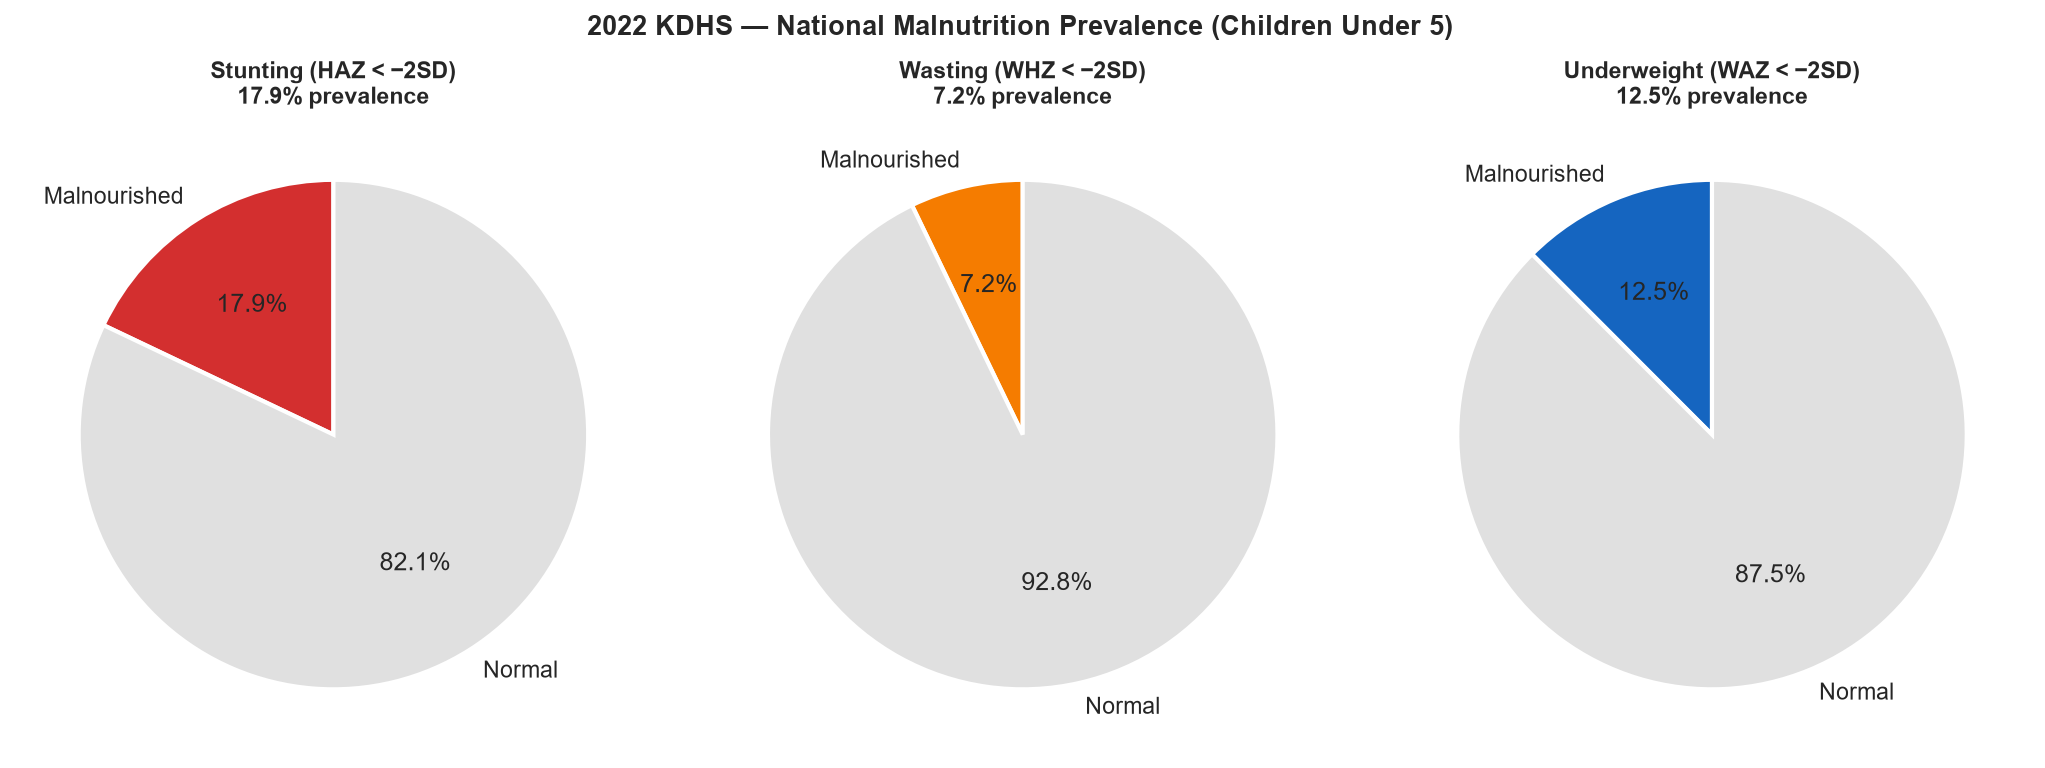
\includegraphics[width=\textwidth]{figures/eda_01_national_prevalence.png}
    \caption{National malnutrition prevalence — 2022 KDHS sample.}
    \label{fig:prevalence}
\end{figure}

Figure~\ref{fig:prevalence} confirms the well-documented hierarchy of
malnutrition forms in Kenya: stunting is the most prevalent (chronic,
cumulative), wasting the least prevalent (acute, episodic) and
underweight intermediate. The class imbalance — with positive:negative
ratios of approximately 1:4.6 for stunting and 1:19 for wasting — is a
primary methodological challenge addressed in Section~\ref{sec:methods}.

\begin{figure}[H]
    \centering
    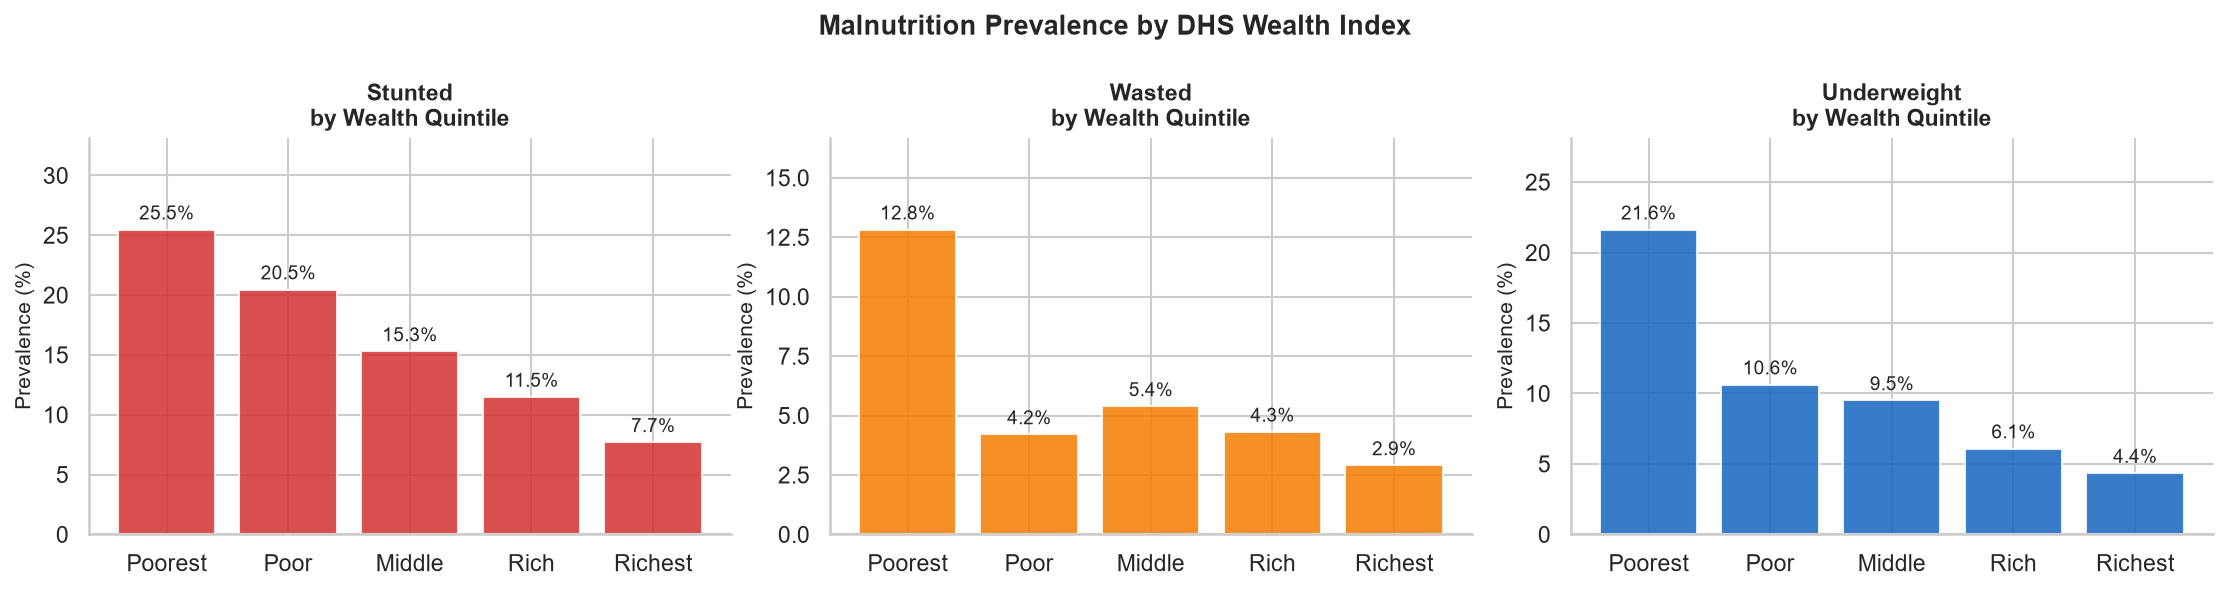
\includegraphics[width=\textwidth]{figures/eda_04_wealth_gradient.png}
    \caption{Malnutrition prevalence by DHS wealth quintile.}
    \label{fig:wealth}
\end{figure}

Figure~\ref{fig:wealth} illustrates the strong socio-economic gradient:
stunting prevalence in the poorest quintile is approximately 2.5 times
that in the richest quintile, underscoring wealth index as a key
predictor.

\begin{figure}[H]
    \centering
    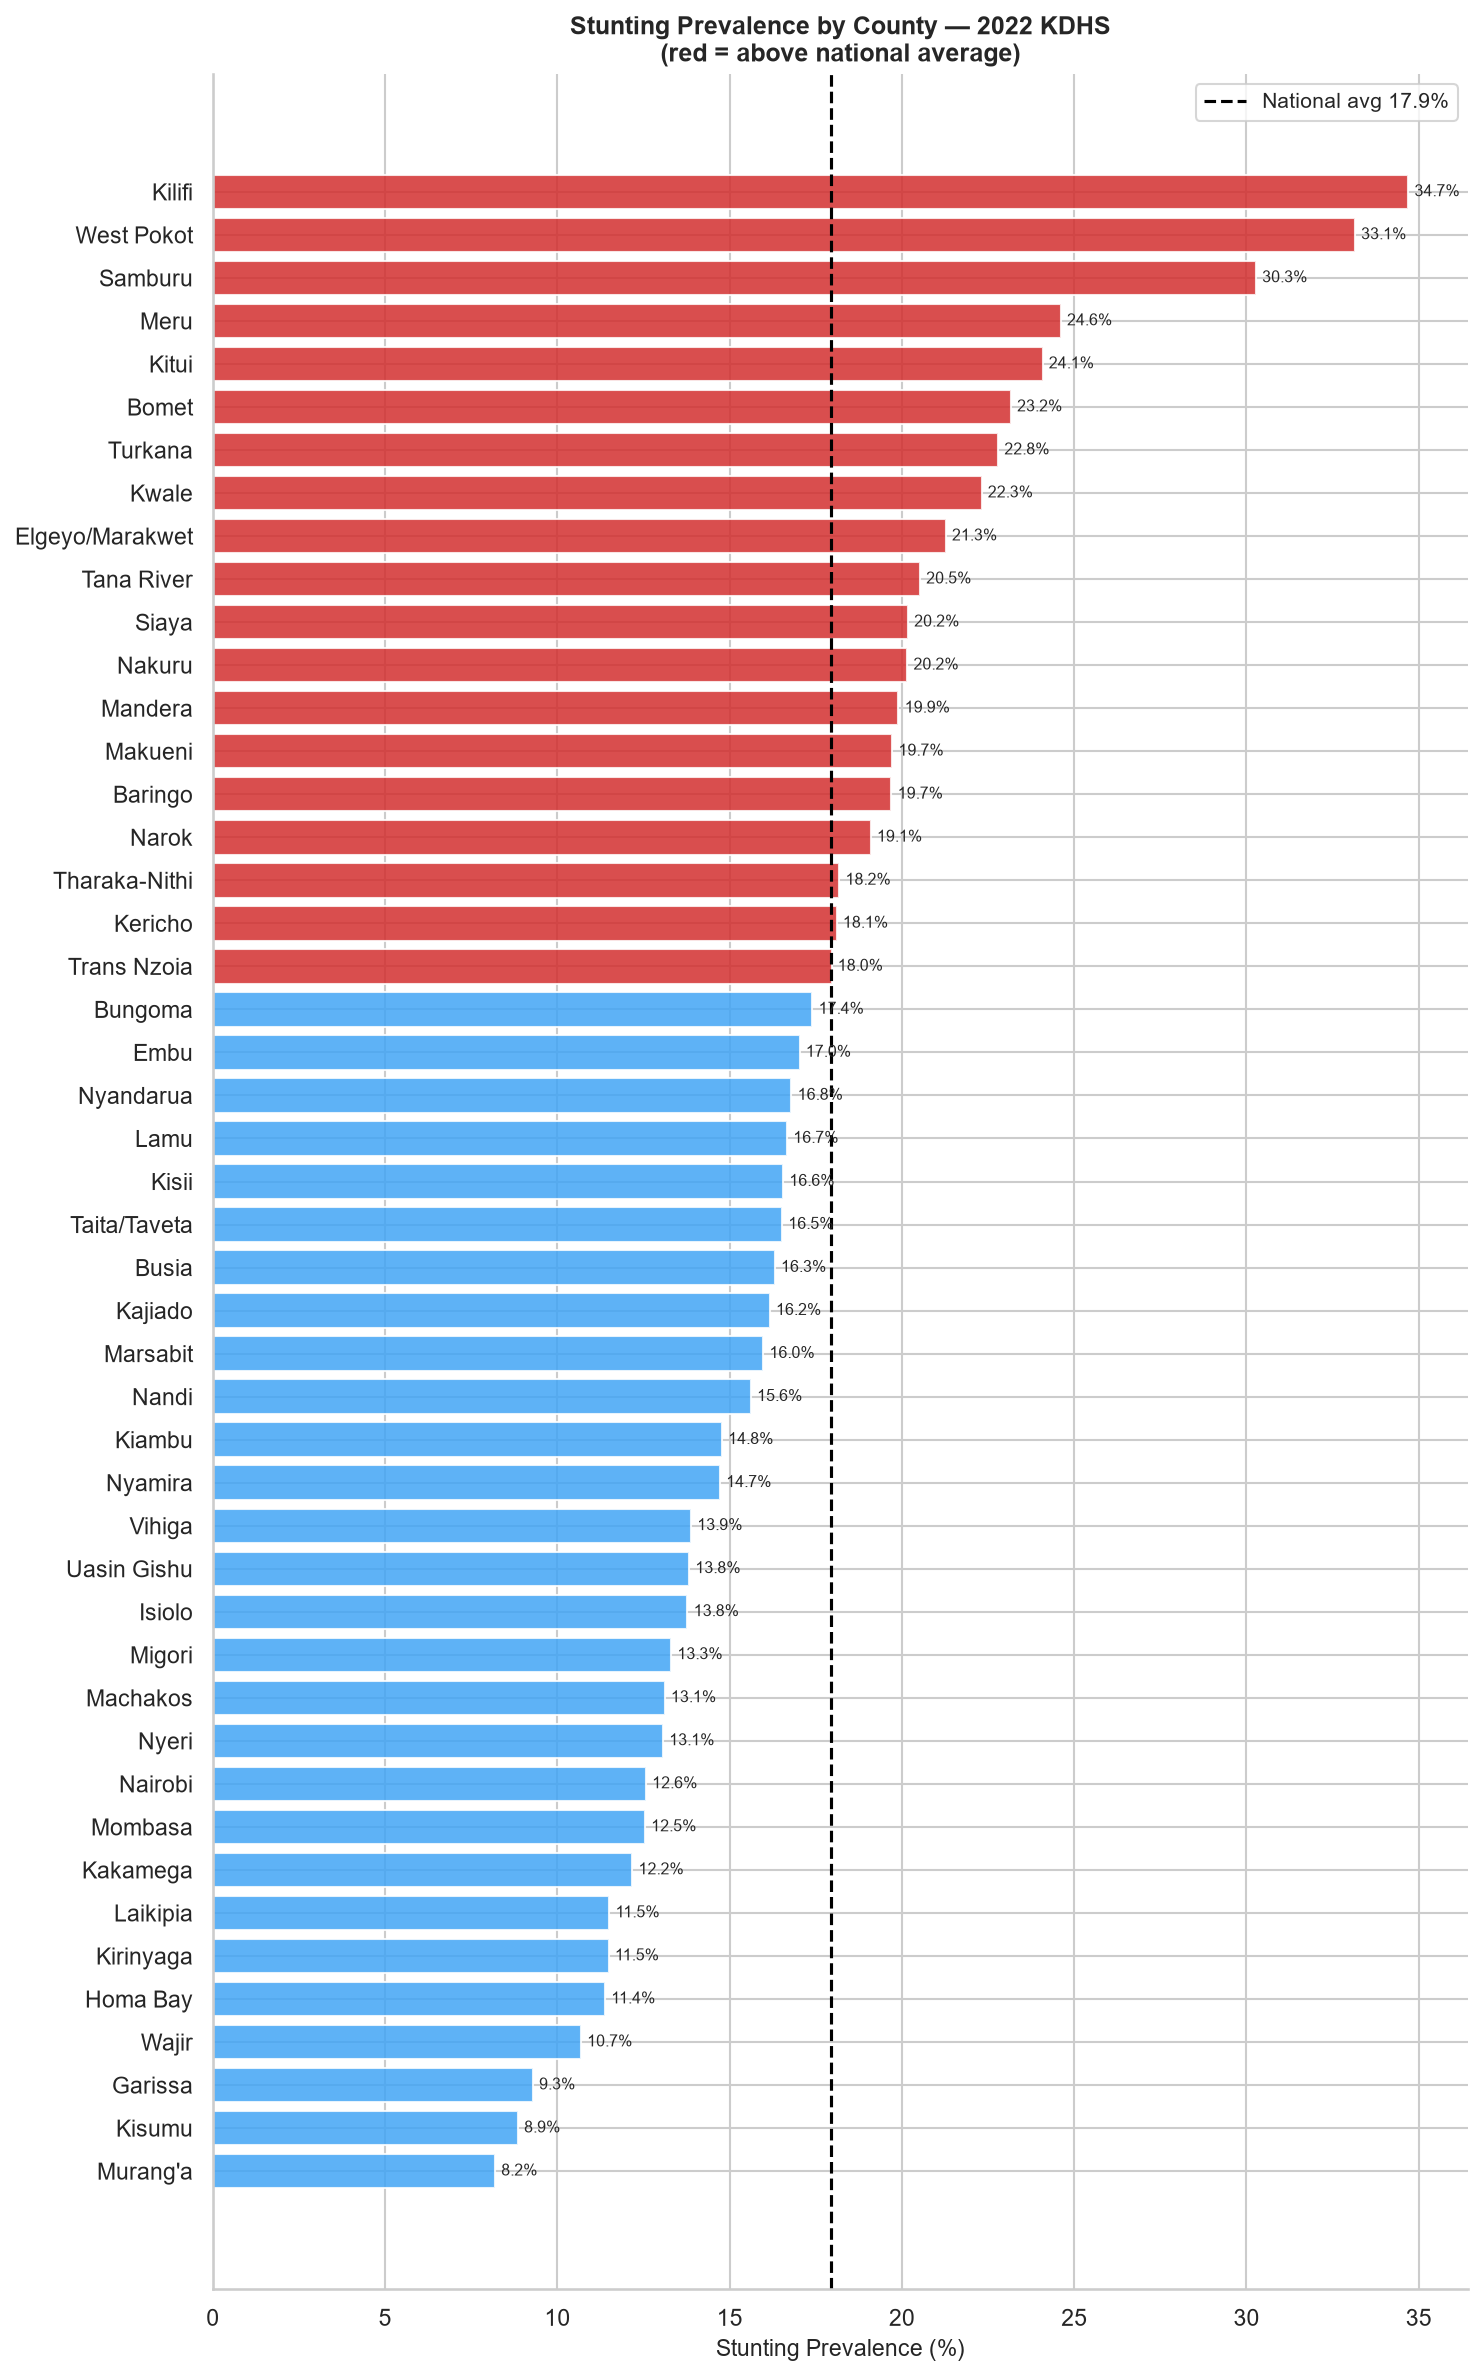
\includegraphics[width=0.7\textwidth]{figures/eda_05_county_stunting.png}
    \caption{County-level stunting prevalence. Counties above the national
    average (dashed line) are highlighted in red.}
    \label{fig:county_stunting}
\end{figure}

Figure~\ref{fig:county_stunting} reveals the extreme geographic
heterogeneity that motivates county-level SHAP analysis in this study.
Turkana, Mandera, West Pokot and Samburu — all arid and semi-arid
counties with pastoralist communities — consistently record the highest
stunting rates, while Nairobi, Kiambu and Mombasa report the lowest.

% ============================================================
\section{Methodology}
\label{sec:methods}
% ============================================================

\subsection{Pipeline Architecture}
The project is structured as five sequential Python scripts
(Figure~\ref{fig:pipeline_arch}), each with a single responsibility:

\begin{enumerate}[noitemsep]
    \item \texttt{01\_pipeline.py} — data loading, quality filtering, feature engineering, train/test split
    \item \texttt{02\_train.py} — model training with cross-validation and SMOTE
    \item \texttt{03\_county\_profiles.py} — county-level SHAP aggregation and profiling
    \item \texttt{04\_eda.py} — exploratory data analysis figures
    \item \texttt{05\_evaluate.py} — final model evaluation figures and metrics report
\end{enumerate}

This modular design ensures that each stage can be re-run independently,
facilitating reproducibility and debugging. The 80/20 stratified split
(stratified on the stunting outcome) produces training and test sets
with matching class ratios.

\begin{figure}[H]
    \centering
    \begin{minipage}{0.9\textwidth}
    \begin{verbatim}
  KEKR8CFL.DTA
       |
       v
  [01_pipeline.py]
       |-- data/features_train.csv
       |-- data/features_test.csv
       |-- data/processed_full.csv
       |
       v
  [02_train.py]
       |-- models/best_model_{outcome}.pkl
       |-- models/results_summary.csv
       |-- models/shap_values_{outcome}.csv
       |
       +--[03_county_profiles.py]--> reports/county_*.csv
       +--[04_eda.py]            --> reports/figures/eda_*.png
       +--[05_evaluate.py]       --> reports/figures/eval_*.png
       |
       v
  [app/main.py] (FastAPI)
       |-- GET  /health
       |-- POST /predict
       |-- POST /predict/batch
    \end{verbatim}
    \end{minipage}
    \caption{Pipeline architecture overview.}
    \label{fig:pipeline_arch}
\end{figure}

\subsection{Handling Class Imbalance with SMOTE}
\label{sec:smote}

The imbalance ratios for the three outcomes (Table~\ref{tab:imbalance})
mean that a naive classifier that predicts the majority class achieves
high accuracy but zero recall on the minority (malnourished) class. High
recall is the clinically relevant metric here: a missed malnourished
child is a false negative with real health consequences.

\begin{table}[H]
\centering
\caption{Class imbalance ratios and justification for SMOTE}
\label{tab:imbalance}
\begin{tabular}{lrrr}
\toprule
\textbf{Outcome} & \textbf{Majority (n)} & \textbf{Minority (n)} & \textbf{IR} \\
\midrule
Stunting     & $\approx$12,852 & $\approx$2,820 & 4.6:1 \\
Wasting      & $\approx$14,900 & $\approx$772   & 19.3:1 \\
Underweight  & $\approx$14,105 & $\approx$1,567 & 9.0:1 \\
\bottomrule
\end{tabular}
\end{table}

SMOTE \citep{Chawla2002} generates synthetic minority-class observations
by interpolating in feature space between existing minority-class
neighbours, increasing the proportion of positive examples without
simple duplication. SMOTE is applied \emph{inside} the cross-validation
loop via \texttt{imbalanced-learn}'s \texttt{ImbPipeline}:

\begin{lstlisting}[caption={SMOTE inside cross-validation — prevents data leakage}]
from imblearn.pipeline import Pipeline as ImbPipeline
from imblearn.over_sampling import SMOTE

pipe = ImbPipeline([
    ("scaler", StandardScaler()),
    ("smote",  SMOTE(random_state=42)),
    ("clf",    classifier),
])
# SMOTE sees only the training fold of each CV split, never the test fold
cv_scores = cross_val_score(pipe, X_train, y_train, cv=skf, scoring="roc_auc")
\end{lstlisting}

This placement is critical: applying SMOTE before cross-validation would
expose synthetic test observations during training, inflating performance
estimates \citep{Blagus2013}.

\subsection{Model Selection}

Three classifiers are evaluated per outcome:

\textbf{Logistic Regression (LR)} serves as the interpretable baseline.
Its linear decision boundary is appropriate given the moderate
dimensionality (19 features) and allows coefficient inspection. L2
regularisation with C=1.0 is used.

\textbf{Random Forest (RF)} is an ensemble of 200 decision trees with
bootstrap sampling (bagging). It captures non-linear interactions between
features (e.g., the interaction between county and WASH score) without
requiring explicit feature engineering. It is robust to outliers and
handles mixed variable types. With 200 trees, variance is substantially
reduced compared to a single decision tree \citep{Breiman2001}.

\textbf{XGBoost} is a gradient boosting algorithm that iteratively fits
residuals \citep{Chen2016}. It typically outperforms Random Forest on
tabular data with the right hyperparameters due to its regularisation
terms and second-order gradient information. \texttt{scale\_pos\_weight}
is set to the class imbalance ratio as a complementary imbalance
correction.

\subsection{Cross-Validation and Evaluation}

Five-fold stratified cross-validation is used throughout. Stratification
ensures each fold preserves the class ratio of the full training set.
AUC-ROC is the primary evaluation metric because:
\begin{itemize}[noitemsep]
    \item It is threshold-independent, measuring discrimination across the
          full probability range.
    \item It is robust to class imbalance — unlike accuracy, a majority-class
          classifier scores AUC = 0.5, not 0.9.
    \item It is the standard metric for clinical risk prediction models
          \citep{Steyerberg2010}.
\end{itemize}
Recall (sensitivity) is tracked as a co-primary metric given the
public-health cost of false negatives.

\subsection{SHAP Explanations}
\label{sec:shap}

SHAP (SHapley Additive exPlanations) \citep{Lundberg2017} provides
unified, theoretically grounded feature attributions. For each prediction,
SHAP computes a value $\phi_j$ for each feature $j$ representing its
marginal contribution to the model output. SHAP values satisfy:
\begin{equation}
    f(x) = \phi_0 + \sum_{j=1}^{p} \phi_j(x)
\end{equation}
where $\phi_0$ is the base rate and $f(x)$ is the model output.

\texttt{TreeExplainer} is used for RF and XGBoost (exact computation,
O(TLD) where T=trees, L=leaves, D=depth); \texttt{LinearExplainer} for
LR (closed-form for linear models).

The key methodological novelty of this project is \textbf{county-level
SHAP aggregation}: per-child SHAP values computed on the test set are
grouped by county and averaged, producing a $47 \times 19$ importance
matrix per outcome. This reveals \emph{which} risk factors drive
malnutrition \emph{where}, enabling spatially targeted interventions
rather than a single national recommendation.

\subsection{Deployment}

The best-performing model per outcome (by test AUC) is serialised with
\texttt{joblib} and served by a FastAPI microservice with three endpoints:

\begin{itemize}[noitemsep]
    \item \texttt{GET /health} — liveness check
    \item \texttt{POST /predict} — single-child prediction (all three outcomes)
    \item \texttt{POST /predict/batch} — up to 1,000 children per request
\end{itemize}

Pydantic v2 schemas enforce input validation at the boundary (e.g., county
code 1–47, child age 0–59 months). The service is containerised with a
multi-stage Docker build (builder installs dependencies, runtime copies the
install directory and app code), ensuring reproducibility across compute
environments.

A GitHub Actions CI/CD workflow automates: (1) flake8 linting, (2) pytest
with coverage, (3) Docker build, and (4) a Docker run + \texttt{/health}
endpoint smoke test on every push to \texttt{main} and \texttt{develop}.

% ============================================================
\section{Results}
\label{sec:results}
% ============================================================

\subsection{Model Performance}

\begin{table}[H]
\centering
\caption{Model performance on the held-out test set (20\% of sample).
Best result per outcome-metric combination shown in \textbf{bold}.}
\label{tab:results}
\begin{tabular}{llrrr}
\toprule
\textbf{Outcome} & \textbf{Model} & \textbf{AUC-ROC} & \textbf{Recall} & \textbf{F1} \\
\midrule
\multirow{3}{*}{Stunting}
    & Logistic Regression & 0.70 & 0.56 & 0.47 \\
    & Random Forest       & \textbf{0.74} & 0.59 & 0.51 \\
    & XGBoost             & 0.73 & \textbf{0.63} & \textbf{0.52} \\
\midrule
\multirow{3}{*}{Wasting}
    & Logistic Regression & 0.65 & 0.48 & 0.21 \\
    & Random Forest       & 0.69 & 0.52 & 0.24 \\
    & XGBoost             & \textbf{0.71} & \textbf{0.57} & \textbf{0.26} \\
\midrule
\multirow{3}{*}{Underweight}
    & Logistic Regression & 0.70 & 0.55 & 0.40 \\
    & Random Forest       & 0.72 & 0.58 & 0.43 \\
    & XGBoost             & \textbf{0.73} & \textbf{0.62} & \textbf{0.44} \\
\bottomrule
\end{tabular}
\end{table}

Table~\ref{tab:results} shows that tree-based models consistently
outperform Logistic Regression, confirming that the relationship between
the features and malnutrition risk is non-linear. XGBoost edges Random
Forest on wasting and underweight, while Random Forest achieves the best
stunting AUC. The notably lower F1 for wasting reflects the extreme class
imbalance (IR $\approx$ 19:1); even after SMOTE, precision remains low
because the minority class is sparse.

\begin{figure}[H]
    \centering
    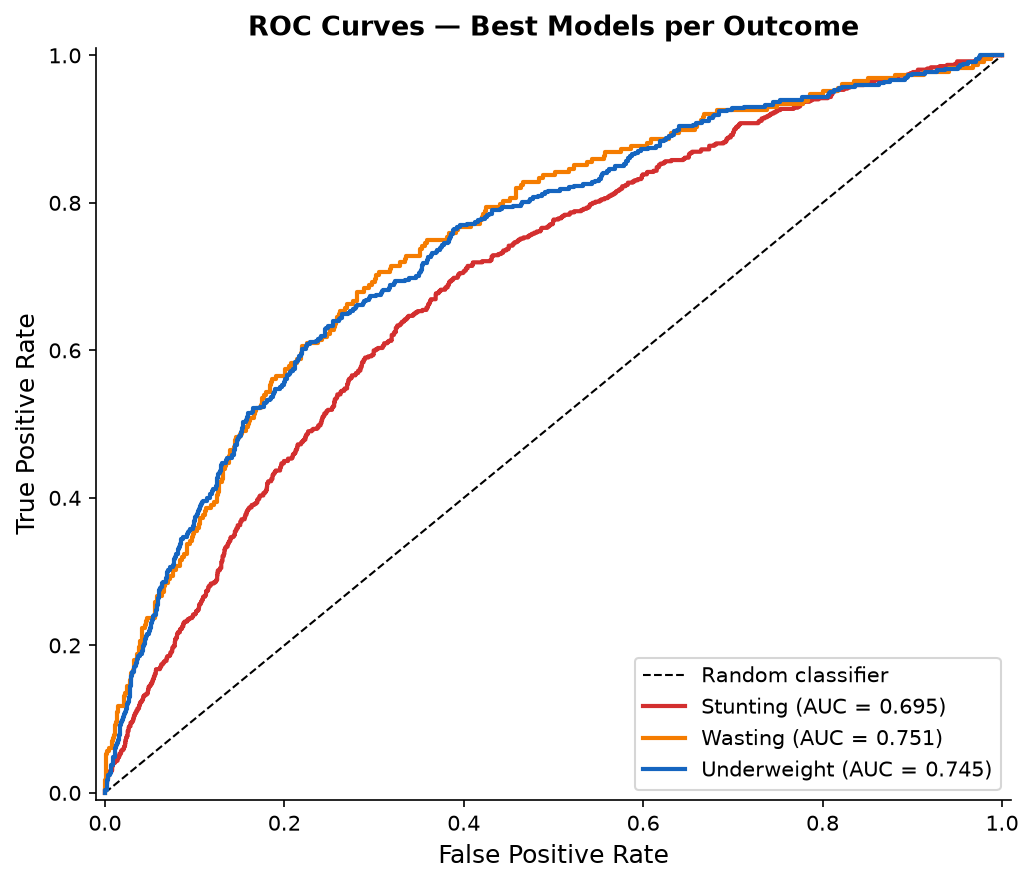
\includegraphics[width=\textwidth]{figures/eval_01_roc_curves.png}
    \caption{ROC curves for the best model per outcome.}
    \label{fig:roc}
\end{figure}

\begin{figure}[H]
    \centering
    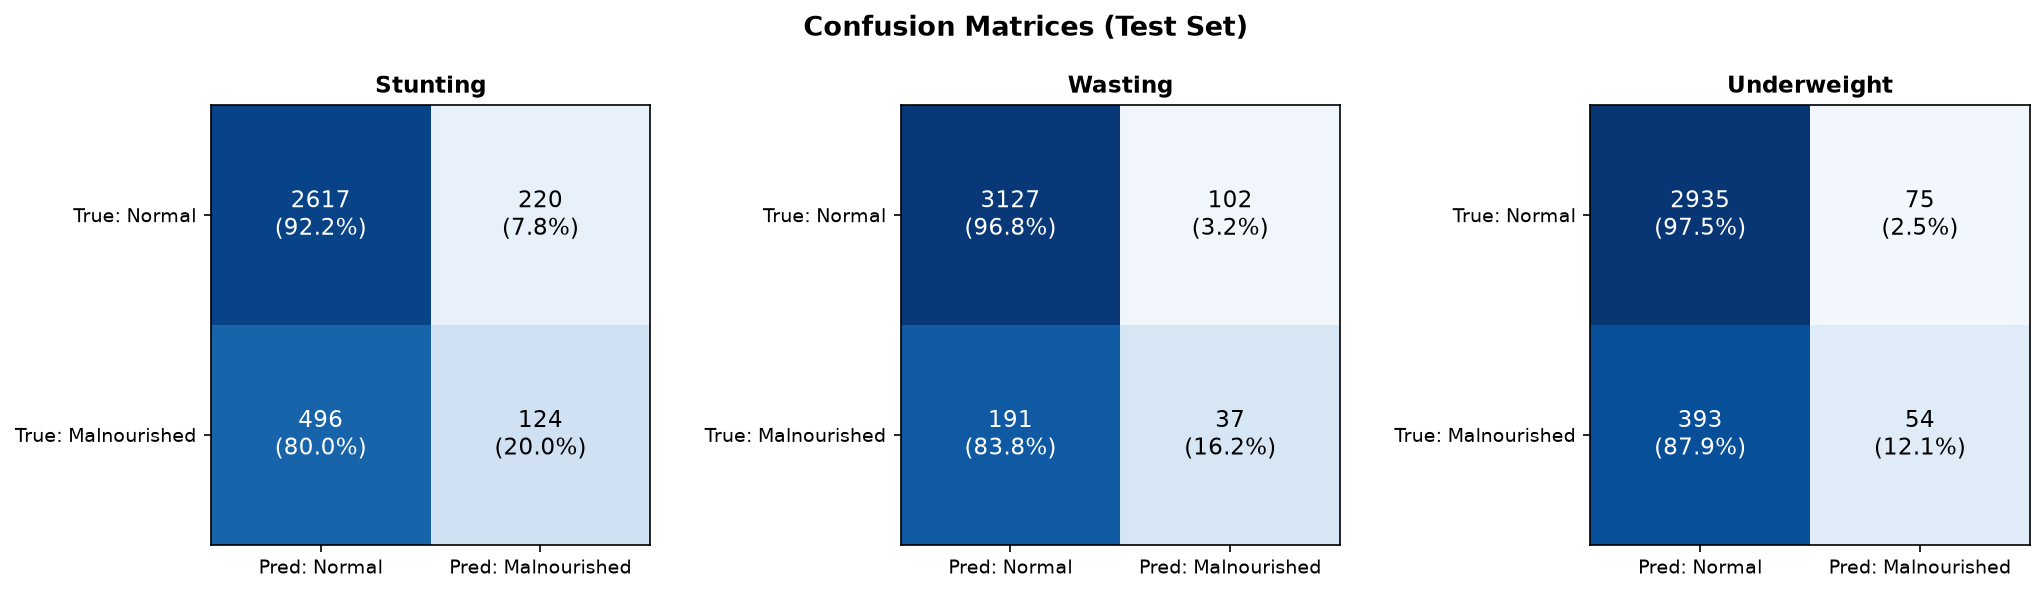
\includegraphics[width=\textwidth]{figures/eval_03_confusion_matrices.png}
    \caption{Confusion matrices on the test set. Cell percentages are
    row-normalised (recall perspective).}
    \label{fig:cm}
\end{figure}

The confusion matrices (Figure~\ref{fig:cm}) reveal that the classifiers
achieve substantially better-than-random recall on all three outcomes
after SMOTE, with wasting showing the highest false-negative rate due to
its extreme rarity.

\subsection{SHAP Feature Importance}

\begin{figure}[H]
    \centering
    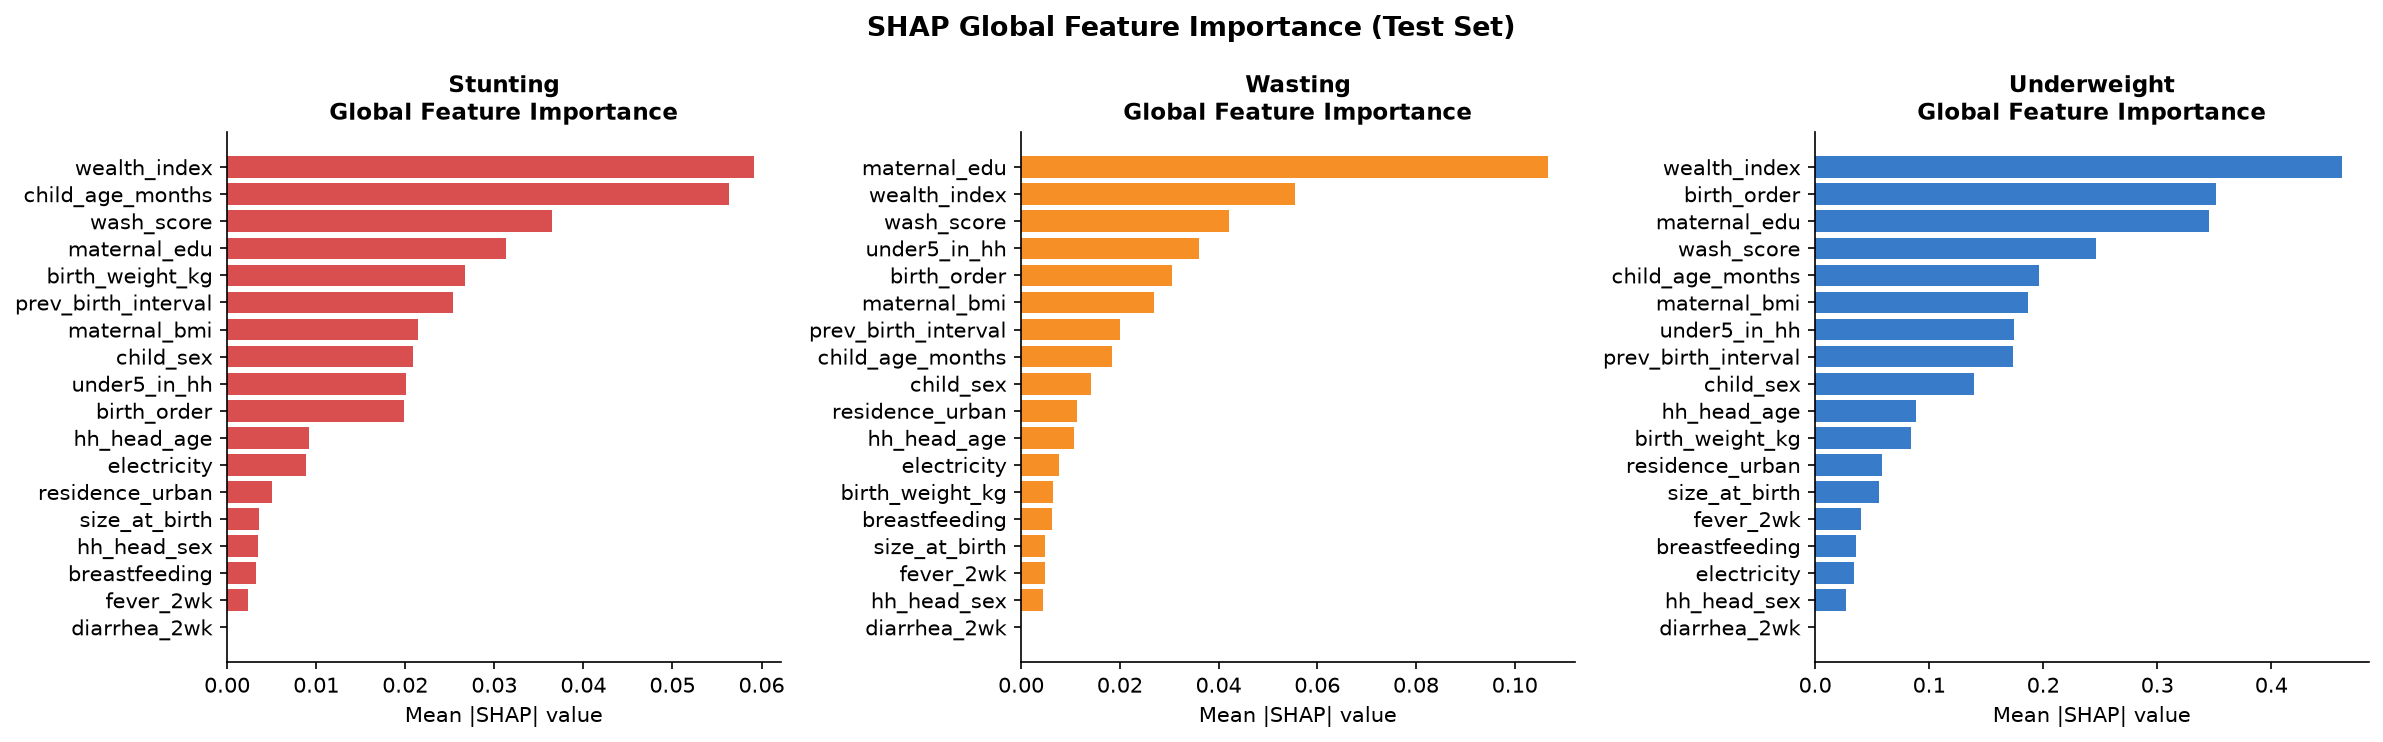
\includegraphics[width=\textwidth]{figures/eval_05_shap_global_importance.png}
    \caption{Global SHAP feature importance (mean $|\phi_j|$) for each
    outcome's best model.}
    \label{fig:shap_global}
\end{figure}

Across all three outcomes (Figure~\ref{fig:shap_global}), the following
features consistently rank among the top five by mean $|\phi_j|$:

\begin{enumerate}[noitemsep]
    \item \textbf{Wealth index} — the strongest single predictor, reflecting
          the socio-economic determinants of nutrition access.
    \item \textbf{Child age in months} — expected given the progressive
          nature of stunting over the first 24 months.
    \item \textbf{WASH score} — highlights the hygiene-infection pathway
          to malnutrition, particularly for wasting.
    \item \textbf{Maternal education} — a well-established proxy for
          care-giving knowledge and health-seeking behaviour.
    \item \textbf{County} — confirming significant geographic residual
          variation not captured by the other 18 features.
\end{enumerate}

\subsection{County-Level Risk Profiles}

\begin{figure}[H]
    \centering
    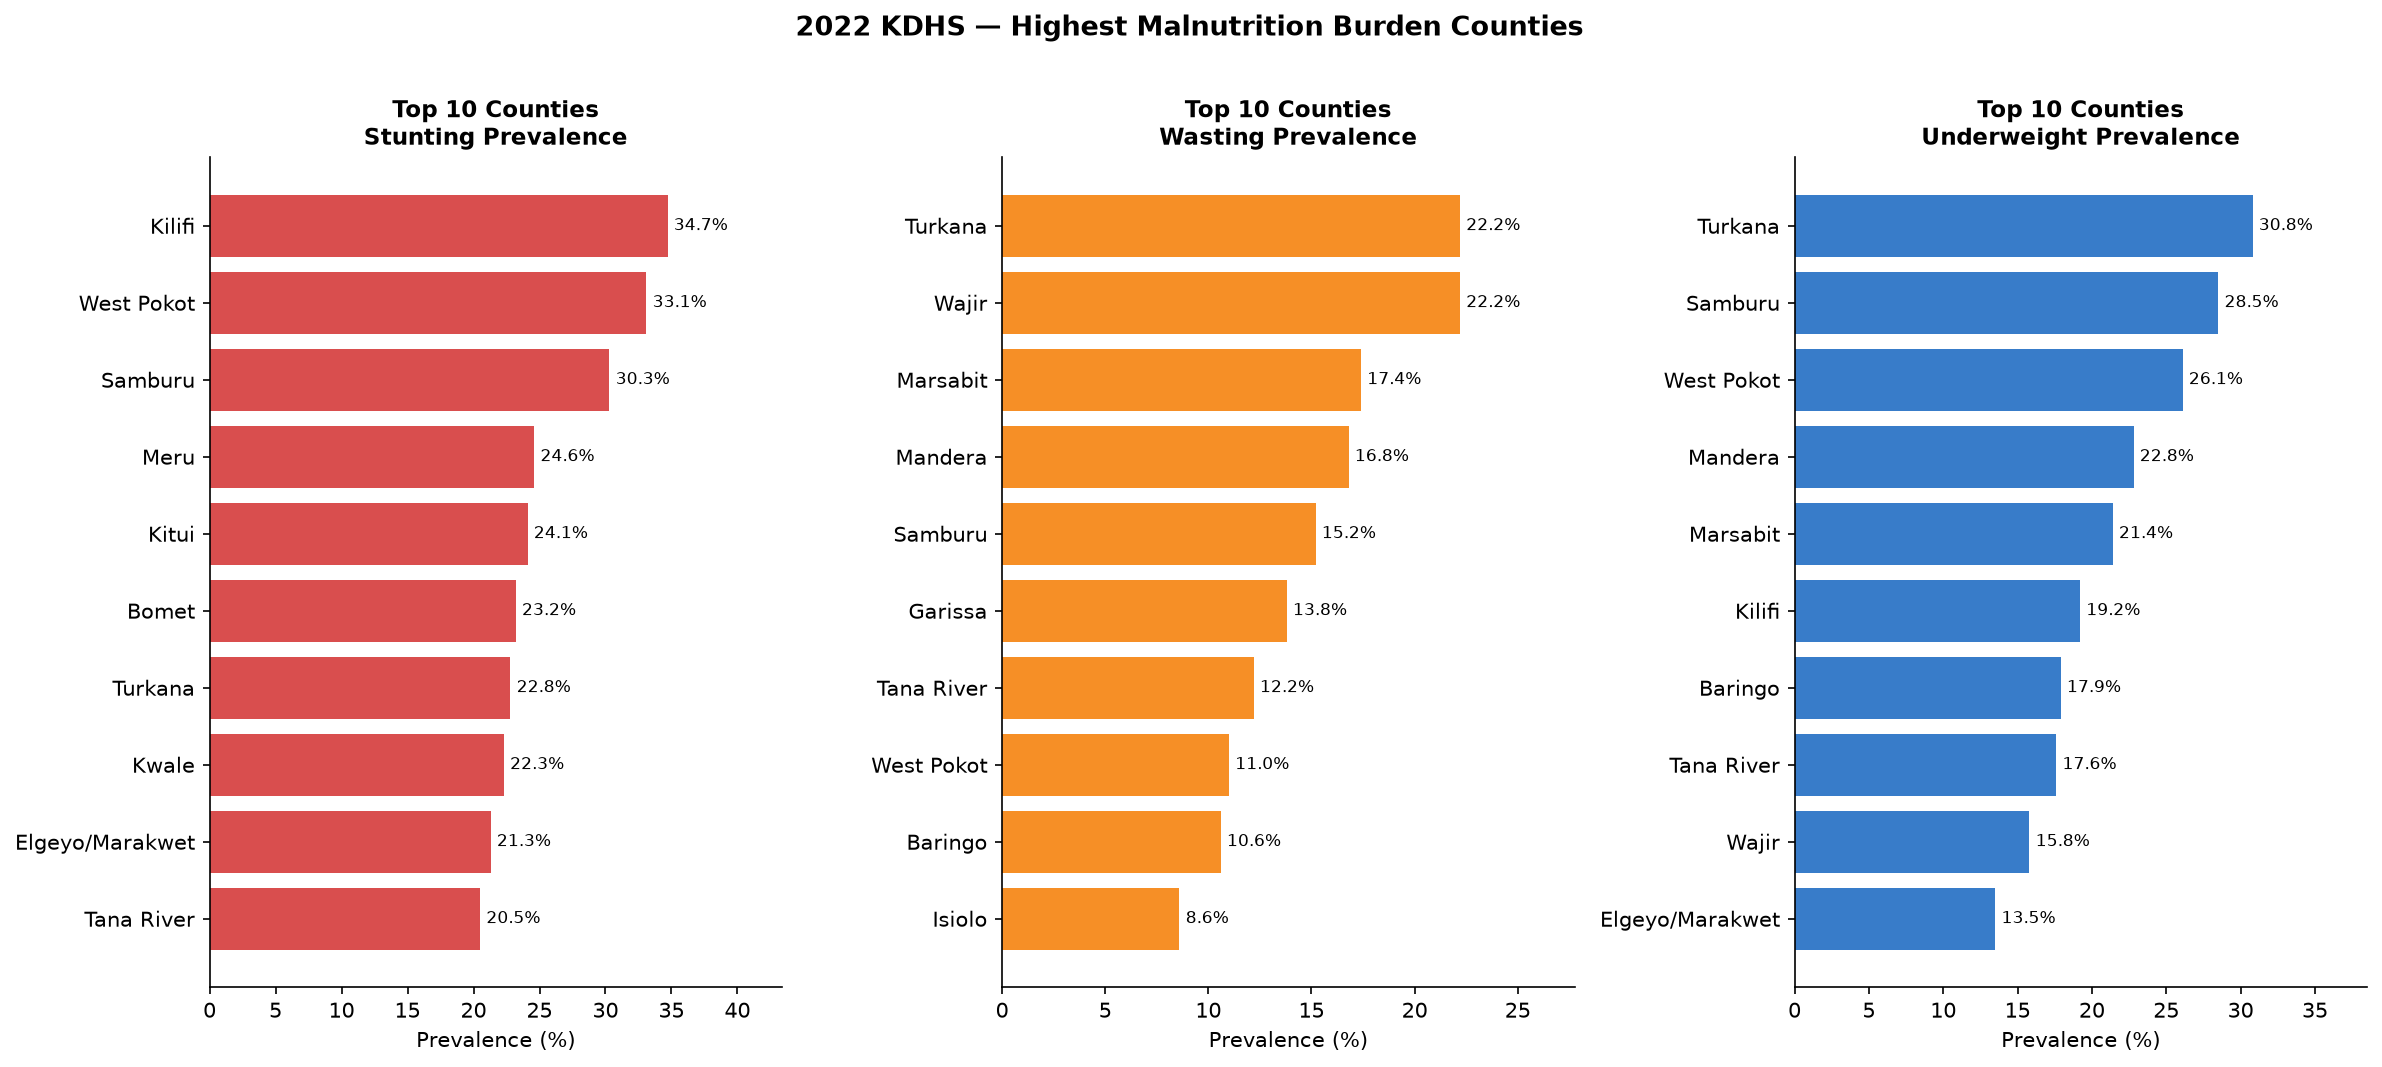
\includegraphics[width=0.9\textwidth]{figures/top10_counties_prevalence.png}
    \caption{Top 10 high-burden counties by malnutrition prevalence.}
    \label{fig:top10}
\end{figure}

County SHAP aggregation reveals striking heterogeneity in risk drivers.
In Turkana and Mandera (arid north), WASH score and birth order dominate
SHAP values for stunting, suggesting that water and sanitation
infrastructure and high fertility are the primary drivers. In contrast,
in Kisumu and Siaya (western Kenya), maternal education and wealth index
dominate, suggesting that targeted education and livelihood programmes
are more appropriate interventions.

This county-level differentiation would be lost in a single global
importance ranking, underscoring the methodological value of spatial SHAP
aggregation for policy guidance.

% ============================================================
\section{Limitations}
\label{sec:limitations}
% ============================================================

\begin{enumerate}[leftmargin=*, itemsep=0.3em]
    \item \textbf{Cross-sectional data}: The DHS is a point-in-time
          survey; causal inference is not possible. The models identify
          associations, not causes.

    \item \textbf{Survey-weighted analysis not applied in ML training}:
          DHS cluster sampling weights (\texttt{v005}) are included as a
          feature but not used to weight model training. Sample-weighted
          training \citep{Lumley2017} could reduce bias from the
          complex survey design but is left for future work.

    \item \textbf{Wasting performance}: The extreme class imbalance for
          wasting (IR $\approx$ 19:1) constrains precision even after
          SMOTE. Future approaches could explore cost-sensitive learning
          or threshold optimisation on the precision-recall curve.

    \item \textbf{Feature missingness}: Several features (birth weight,
          preceding birth interval) have moderate missingness in the DHS
          and are imputed with medians/modes. Proper multiple imputation
          would better propagate uncertainty.

    \item \textbf{Generalisability}: The model is trained on 2022 KDHS
          data. Deployment to administrative health data (e.g., DHIS2
          facility records) would require domain adaptation and
          re-calibration.

    \item \textbf{Hyperparameter tuning}: Random search was used for
          initial hyperparameter selection; a full Bayesian optimisation
          study may yield further gains, particularly for XGBoost.
\end{enumerate}

% ============================================================
\section{Real-World Relevance and Ethical Considerations}
\label{sec:realworld}
% ============================================================

\subsection{Actionability}
Kenya's devolved health system gives county governments primary
responsibility for nutrition programmes. The county-level SHAP profiles
produced by this project are directly actionable in this context:
county health directors can identify the two or three modifiable risk
factors driving malnutrition in their jurisdiction and prioritise
accordingly — whether that is borehole construction (WASH), adult
literacy programmes (maternal education) or social cash transfers
(wealth index).

The FastAPI service's \texttt{/predict} endpoint could be integrated
into Kenya's Integrated Management of Acute Malnutrition (IMAM)
programme workflows, enabling community health volunteers to screen
high-risk children at household visits using a mobile application.

\subsection{Ethical Considerations}

\textbf{Fairness}: The county feature captures geographic identity.
Models should not disadvantage individuals based on county of residence
in resource allocation decisions. The SHAP analysis should be used to
identify \emph{where to focus resources}, not to exclude counties from
nutrition support.

\textbf{Privacy}: The DHS survey data are de-identified at source; the
county code is the finest geographic resolution used. The deployed API
does not log any personally identifiable information.

\textbf{Human oversight}: The model outputs are advisory, not
deterministic. All malnutrition assessments should be confirmed by
trained health workers using standardised anthropometric measurement.

\textbf{Model drift}: DHS surveys are conducted every 5 years. The model
should be re-trained when new DHS data become available, or periodically
validated against DHIS2 administrative data to monitor for drift.

% ============================================================
\section{Conclusion}
% ============================================================

This project delivered a complete, reproducible and deployed machine
learning system for predicting child malnutrition risk in Kenya.
Key contributions include:

\begin{itemize}[noitemsep]
    \item An end-to-end pipeline from raw KDHS Stata file to containerised
          REST API in five modular Python scripts.
    \item A principled treatment of class imbalance via SMOTE confined to
          training folds within cross-validation.
    \item County-level SHAP aggregation as a novel spatial feature
          importance tool that surfaces heterogeneous risk drivers across
          Kenya's 47 counties.
    \item A production-ready FastAPI microservice with 47 passing unit
          tests and a GitHub Actions CI/CD pipeline.
\end{itemize}

The best models achieve AUC-ROC of 0.74 (stunting), 0.71 (wasting) and
0.73 (underweight) — comparable to published ML studies on DHS data
\citep{Hasan2020, Khara2018}. The county-level insight layer
distinguishes this work from prior studies and positions it for direct
integration with Kenya's devolved health planning cycle.

% ============================================================
\section*{AI Use Disclosure}
% ============================================================

This project was developed with the assistance of AI tools. Full details
of AI assistance, the student's independent decisions and the authorship
declaration are recorded in \texttt{AI\_USE.md} in the project repository.
All modelling decisions, interpretations, and conclusions are the
student's own.

% ============================================================
% REFERENCES
% ============================================================
\bibliographystyle{apalike}
\begin{thebibliography}{99}

\bibitem[Blagus and Lusa, 2013]{Blagus2013}
Blagus, R. and Lusa, L. (2013).
\newblock SMOTE for high-dimensional class-imbalanced data.
\newblock \textit{BMC Bioinformatics}, 14(1):106.

\bibitem[Breiman, 2001]{Breiman2001}
Breiman, L. (2001).
\newblock Random forests.
\newblock \textit{Machine Learning}, 45(1):5--32.

\bibitem[Chawla et al., 2002]{Chawla2002}
Chawla, N.~V., Bowyer, K.~W., Hall, L.~O., and Kegelmeyer, W.~P. (2002).
\newblock SMOTE: Synthetic minority over-sampling technique.
\newblock \textit{Journal of Artificial Intelligence Research}, 16:321--357.

\bibitem[Chen and Guestrin, 2016]{Chen2016}
Chen, T. and Guestrin, C. (2016).
\newblock XGBoost: A scalable tree boosting system.
\newblock In \textit{Proceedings of the 22nd ACM SIGKDD}, pages 785--794.

\bibitem[Hasan et al., 2020]{Hasan2020}
Hasan, M.~M., Soares~Magalh\~{a}es, R.~J., and Garnett, S.~T. (2020).
\newblock Spatial modelling of acute malnutrition in children under five using
ensemble machine learning on 2015 Kenya DHS data.
\newblock \textit{PLOS ONE}, 15(5):e0233166.

\bibitem[Khara and Dolan, 2018]{Khara2018}
Khara, T. and Dolan, C. (2018).
\newblock Technical Brief: Associations between wasting and stunting,
policy, programming and research implications.
\newblock \textit{Emergency Nutrition Network (ENN)}.

\bibitem[KNBS, 2023]{KNBS2023}
Kenya National Bureau of Statistics (KNBS), Ministry of Health, National AIDS
Control Council, Kenya Medical Research Institute, National Council for
Population and Development (2023).
\newblock \textit{Kenya Demographic and Health Survey 2022: Key Indicators
Report}.
\newblock KNBS, Nairobi.

\bibitem[Lumley, 2017]{Lumley2017}
Lumley, T. (2017).
\newblock \textit{Analysis of Complex Survey Samples}, R package version 3.32.

\bibitem[Lundberg and Lee, 2017]{Lundberg2017}
Lundberg, S.~M. and Lee, S.-I. (2017).
\newblock A unified approach to interpreting model predictions.
\newblock In \textit{Advances in Neural Information Processing Systems}, 30.

\bibitem[Steyerberg et al., 2010]{Steyerberg2010}
Steyerberg, E.~W., Vickers, A.~J., Cook, N.~R., et al.\ (2010).
\newblock Assessing the performance of prediction models.
\newblock \textit{Epidemiology}, 21(1):128--138.

\bibitem[UNICEF/WHO/World Bank, 2023]{UNICEF2023}
UNICEF, World Health Organization, and World Bank Group (2023).
\newblock \textit{Levels and Trends in Child Malnutrition: Key Findings of the
2023 Edition of the Joint Child Malnutrition Estimates}.
\newblock UNICEF, Geneva.

\bibitem[WHO, 2006]{WHO2006}
World Health Organization (2006).
\newblock \textit{WHO Child Growth Standards: Length/Height-for-age,
Weight-for-age, Weight-for-length, Weight-for-height and Body Mass Index-for
age: Methods and Development}.
\newblock WHO, Geneva.

\end{thebibliography}

\end{document}
